\definecolor{deeppeach}{rgb}{1.0, 0.8, 0.64}

\newcommand{\mcell}[1]{\makecell{~\\[-1.05cm]\makebox[0pt]{#1}}}
\newcommand{\graytext}[1]{\color{gray} #1}
\newcommand{\bluetext}[1]{\bf \cellcolor{blue!25} #1}
\newcommand{\redtext}[1]{\bf \cellcolor{red!25} #1}

\newcolumntype{M}[1]{>{\centering\arraybackslash}m{#1}}
\newcolumntype{G}{>{\columncolor{deeppeach!25}\centering\arraybackslash}m{0.08\linewidth}}
\newcolumntype{S}{>{\columncolor{gray!15}\centering\arraybackslash}M{0.10\linewidth}}
\newcommand\setrowheight{\rule{0pt}{1cm}}
\newcolumntype{g}{>{\columncolor{gray!25}\centering\arraybackslash}c}

\begin{table*}[h!]
    \centering
    \begin{tabular}{
        c
        g
        |S|
        G
        M{0.08\linewidth}
        M{0.08\linewidth}
        M{0.08\linewidth}
        ||G
        M{0.08\linewidth}
    }
        & \rotatebox{0}{\bf \large QOS metric} &
        \rotatebox{0}{\bf \large statistic} &
        \rotatebox{60}{\textit{baseline}} &
        \rotatebox{60}{\textit{$\Rightarrow$ multithread}} &
        \rotatebox{60}{\textit{$\Rightarrow$ intranode}} &
        \rotatebox{60}{\textit{+ compute}} &
        \rotatebox{60}{\textit{baseline}} &
        \rotatebox{60}{\textit{+ faulty hw}} \\
        \hline\hline
        \setrowheight
        \multirow[b]{3}{*}{\rotatebox[origin=c]{90}{Updatee Period}} &
            & \mcell{$\Delta$ median} &
            \mcell{XX} &
            \bluetext{\mcell{-XX\%}} &
            \redtext{\mcell{\texttt{+}XX\%}} &
            \graytext{\mcell{+XX\%}} &
            \mcell{XX} &
            \mcell{XX\%} \\ \setrowheight

        &
            & \mcell{\% outliers} &
            \mcell{XX\%} &
            \graytext{\mcell{XX\%}} &
            \graytext{\mcell{XX\%}} &
            \redtext{\mcell{XX\%}} &
            \mcell{XX\%} &
            \mcell{XX\%} \\ \setrowheight

        & \multirow[t]{3}{*}{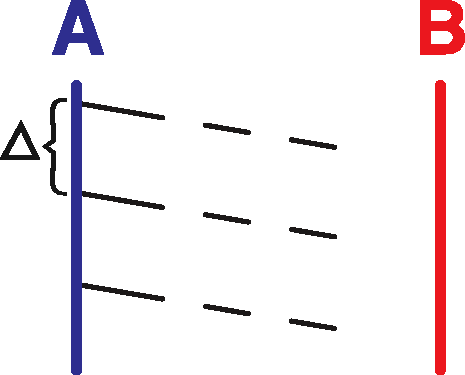
\includegraphics[height=3cm]{img/quality-of-service-metric-definitions/simstep-period-right.pdf}} &
            \mcell{$\sim \mathrm{MAD}$} &
            \mcell{XX\%} &
            \bluetext{\mcell{XX\%}} &
            \graytext{\mcell{XX\%}} &
            \graytext{\mcell{XX\%}} &
            \mcell{XX\%} &
            \mcell{XX\%} \\
        \hline
        \setrowheight
        \multirow[t]{3}{*}{\rotatebox[origin=c]{90}{Walltime Latency~~~~~~~~~~~~~~}} &
            & \mcell{$\Delta$ median} &
            \mcell{XX} &
            \bluetext{\mcell{-XX\%}} &
            \redtext{\mcell{\texttt{+}XX\%}} &
            \graytext{\mcell{+XX\%}} &
            \mcell{XX} &
            \mcell{XX\%} \\ \setrowheight

        &
            & \mcell{\% outliers} &
            \mcell{XX\%} &
            \graytext{\mcell{XX\%}} &
            \graytext{\mcell{XX\%}} &
            \redtext{\mcell{XX\%}} &
            \mcell{XX\%} &
            \mcell{XX\%} \\ \setrowheight

        & \multirow[t]{3}{*}{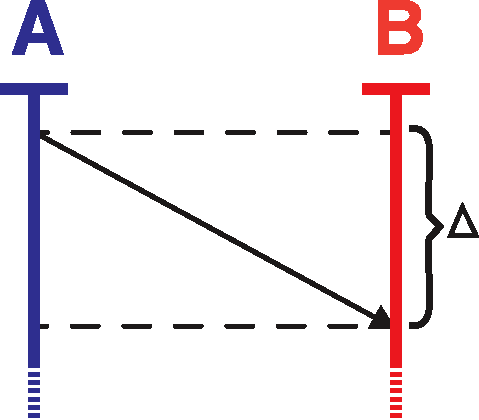
\includegraphics[height=3cm]{img/quality-of-service-metric-definitions/latency-right.pdf}} &
            \mcell{$\sim \mathrm{MAD}$} &
            \mcell{XX\%} &
            \bluetext{\mcell{XX\%}} &
            \graytext{\mcell{XX\%}} &
            \graytext{\mcell{XX\%}} &
            \mcell{XX\%} &
            \mcell{XX\%} \\
        \hline
        \setrowheight
        \multirow[t]{3}{*}{\rotatebox[origin=c]{90}{Updates Latency~~~~~~~~~~~~~~}} &
            & \mcell{$\Delta$ median} &
            \mcell{XX} &
            \bluetext{\mcell{-XX\%}} &
            \redtext{\mcell{\texttt{+}XX\%}} &
            \graytext{\mcell{+XX\%}} &
            \mcell{XX} &
            \mcell{XX\%} \\ \setrowheight

        &
            & \mcell{\% outliers} &
            \mcell{XX\%} &
            \graytext{\mcell{XX\%}} &
            \graytext{\mcell{XX\%}} &
            \redtext{\mcell{XX\%}} &
            \mcell{XX\%} &
            \mcell{XX\%} \\ \setrowheight

        & \multirow[t]{3}{*}{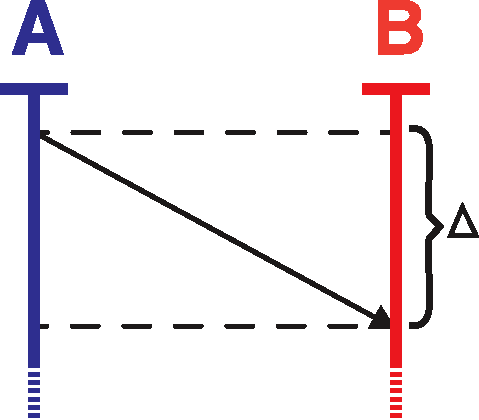
\includegraphics[height=3cm]{img/quality-of-service-metric-definitions/latency-right.pdf}} &
            \mcell{$\sim \mathrm{MAD}$} &
            \mcell{XX\%} &
            \bluetext{\mcell{XX\%}} &
            \graytext{\mcell{XX\%}} &
            \graytext{\mcell{XX\%}} &
            \mcell{XX\%} &
            \mcell{XX\%} \\
        \hline
        \setrowheight
        \multirow[b]{3}{*}{\rotatebox[origin=c]{90}{Bunching}} &
            & \mcell{$\Delta$ median} &
            \mcell{XX} &
            \bluetext{\mcell{-XX\%}} &
            \redtext{\mcell{\texttt{+}XX\%}} &
            \graytext{\mcell{+XX\%}} &
            \mcell{XX} &
            \mcell{XX\%} \\ \setrowheight

        &
            & \mcell{\% outliers} &
            \mcell{XX\%} &
            \graytext{\mcell{XX\%}} &
            \graytext{\mcell{XX\%}} &
            \redtext{\mcell{XX\%}} &
            \mcell{XX\%} &
            \mcell{XX\%} \\ \setrowheight

        & \multirow[t]{3}{*}{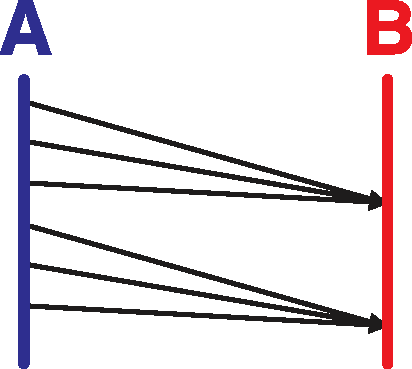
\includegraphics[height=3cm]{img/quality-of-service-metric-definitions/clumpiness-right.pdf}} &
            \mcell{$\sim \mathrm{MAD}$} &
            \mcell{XX\%} &
            \bluetext{\mcell{XX\%}} &
            \graytext{\mcell{XX\%}} &
            \graytext{\mcell{XX\%}} &
            \mcell{XX\%} &
            \mcell{XX\%} \\
        \hline
        \setrowheight
        \multirow[t]{3}{*}{\rotatebox[origin=c]{90}{Delivery Fail Rate~~~~~~~~~~~~~~}} &
            & \mcell{$\Delta$ median} &
            \mcell{XX} &
            \bluetext{\mcell{-XX\%}} &
            \redtext{\mcell{\texttt{+}XX\%}} &
            \graytext{\mcell{+XX\%}} &
            \mcell{XX} &
            \mcell{XX\%} \\ \setrowheight

        &
            & \mcell{\% outliers} &
            \mcell{XX\%} &
            \graytext{\mcell{XX\%}} &
            \graytext{\mcell{XX\%}} &
            \redtext{\mcell{XX\%}} &
            \mcell{XX\%} &
            \mcell{XX\%} \\ \setrowheight

        & \multirow[t]{3}{*}{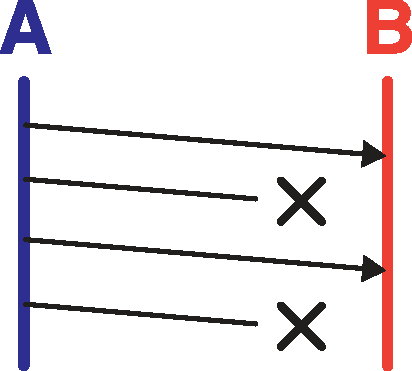
\includegraphics[height=3cm]{img/quality-of-service-metric-definitions/delivery-failure-rate-right.pdf}} &
            \mcell{$\sim \mathrm{MAD}$} &
            \mcell{XX\%} &
            \bluetext{\mcell{XX\%}} &
            \graytext{\mcell{XX\%}} &
            \graytext{\mcell{XX\%}} &
            \mcell{XX\%} &
            \mcell{XX\%} \\
        \hline

    \end{tabular}
    \caption{TODO}
    \label{tab:categorical-composite}
\end{table*}
